% -*-mode: Latex-*-
% !TEX root = kampf.tex
% authors: simon maurer
%
% file: bSF.tex
% contents: Passive SFs des bewaffneten Kampfes
% Sccs-Id: %W% %G%

%==============================================================================
\section{Sonderfertigkeiten für den bewaffneten Kampf}
Folgende Abbildung gibt eine Übersicht über alle Sonderfertigkeiten (mit
AP-Kosten und Voraussetzungen), die im bewaffneten Kampf eingesetzt werden
können. Es handelt sich dabei nicht um die Manöver. Diese werden in den
Kapiteln \ref{chap.bAT} und \ref{chap.bPA} beschrieben.

\begin{figure}
    \centering
    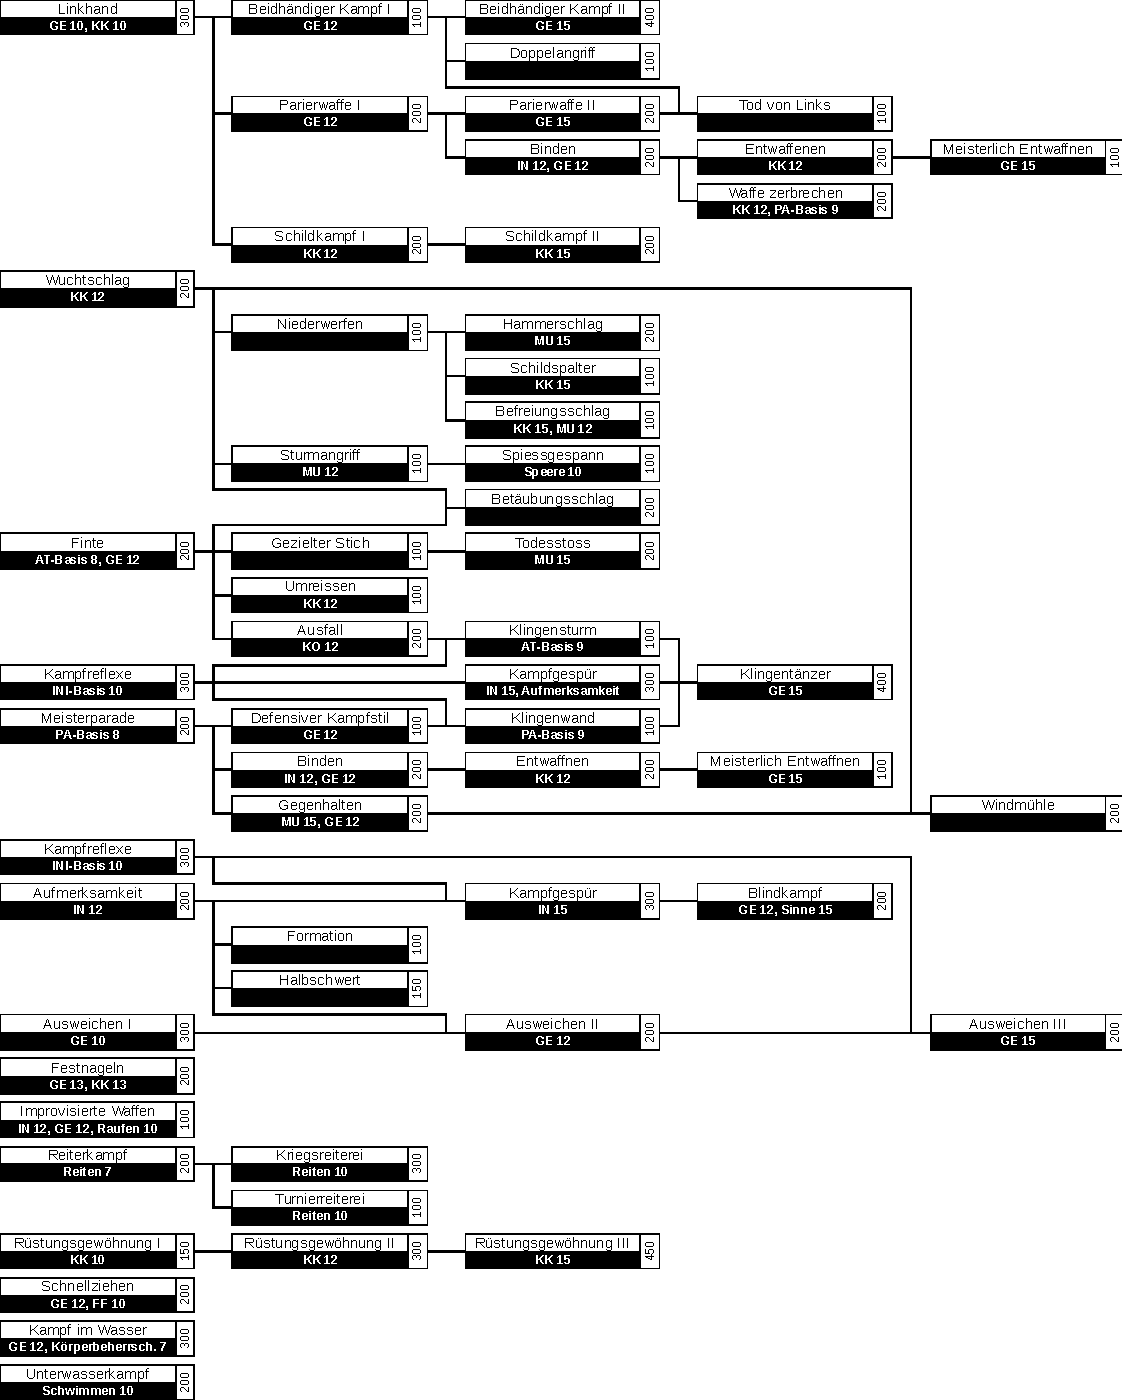
\includegraphics[width=16.986cm,height=21.179cm]{fig/allSF.pdf}
\end{figure}

Im den folgenden Unterkapitel werden Sonderfertigkeiten beschrieben, die nicht
Voraussetzung für ein bestimmtes Manöver sind, sondern einen direkten Einfluss
auf den Kämpfer und seine Fähigkeiten haben.

\subsection{Ausweichen}
Die SFs \textStyleSF{Ausweichen I}, \textStyleSF{Ausweichen II} und
\textStyleSF{Ausweichen III} erhöhen den Ausweichen-Wert um je 3 Punkte. Dieser
Wert berechnet sich aus PA-Basiswert – BE + Boni aus den Sonderfertigkeiten.

Je nach Behinderung ist es möglich zusätzlich zu einer Parade auch noch
Auszuweichen. Siehe Kapitel \ref{chap.A.AW}

\subsection{Aufmerksamkeit}
Gegen einen Kämpfer mit der SF \textStyleSF{Aufmerksamkeit} sind Passierschläge
um 4 Punkte erschwert. Ausserdem ist die IN-Probe um einen Hinterhalt oder eine
Überraschung zu entdecken um 4 Punkte erleichtert.

\subsection{Beidhändiger Kampf}
Mit der SF \textStyleSF{Beidhändiger Kampf I} werden die Abzüge für den Kampf
mit der falschen Hand auf -3 /-3 reduziert und erlaubt zusätzliche Manöver
sowie die Nutzung des KK-Bonus auf die TP der Linken Hand.

Die SF \textStyleSF{Beidhändiger Kampf II} erlaubt alle Abzüge für den Kampf
mit der falsch Hand zu ignorieren und stellt eine zusätzlich Angriffs- oder
Abwehr-Aktion zur Verfügung.

Die Regelung bezüglich der Anzahl Aktionen pro Kampfrunde ist im Kapitel
\ref{chap.A} beschrieben.

\subsection{Blindkampf}
Mit der SF \textStyleSF{Blindkampf} betragen die Abzüge auf AT / PA bei
schlechter oder gar keiner Sicht maximal -2 / -2. Ausserdem ist die IN-Probe um
einen Hinterhalt oder eine Überraschung zu entdecken um weitere 2 Punkte
erleichtert.

\subsection{Halbschwert}
Ein Kämpfer mit der SF \textStyleSF{Halbschwert} kann auch Parieren wenn er
\textStyleSF{Unterlaufen} wurde. Details zum entsprechenden Manöver sind im
Kapitel \ref{chap.bPA.unterlaufen} zu finden.

\subsection{Improvisierte Waffen}
Ein Kenner der SF \textStyleSF{Improvisierte Waffen} kann alle Mali im Kampf
mit improvisierten Waffen ignorieren. Die Waffen werden jedoch auch mit dieser
SF nicht stabiler.

Nachfolgend die Mali für Kämpfer ohne Kenntnis dieser SF:

\begin{itemize}
    \item keine Manöver ausser Wuchtschlag (nur halbe Ansage als Schaden)
    \item Patzer auch bei 19, Prüfwurf um zusätzlich 5 erschwert
    \item Bruchtest bei jeder AT und PA
\end{itemize}

\subsection{Kampfgespür}
Die SF \textStyleSF{Kampfgespür} bringt einen Bonus +2 auf den INI-Wert. Gegen
einen Kämpfer mit dieser SF ist ein Passierschlag um weitere 2 Punkte
erschwert. Ausserdem ist die IN-Probe um einen Hinterhalt oder eine
Überraschung zu entdecken um weitere 4 Punkte erleichtert. Weiter sind die
Manöver \textStyleSF{Klingensturm} und \textStyleSF{Klingenwand} optimaler
einsetzbar (Details siehe Kapitel \ref{chap.bAT.klingensturm} und
\ref{chap.bPA.klingenwand}).

Der Einfluss der Initiative im Kampfgeschehen ist im Kapitel \ref{chap.INI}
beschrieben.

\subsection{Kampfreflexe}
Die SF \textStyleSF{Kampfreflexe} bringt einen Bonus +4 auf den INI-Wert.
Dieser Bonus kommt nur zum Tragen, bei BE kleiner oder gleich 4.

Der Einfluss der Initiative im Kampfgeschehen ist im Kapitel \ref{chap.INI}
beschrieben.

\subsection{Kampf im Wasser}
Mit der SF \textStyleSF{Kampf im Wasser} werden alle Abzüge für den Kampf im
Wasser halbiert.

\subsection{Klingentänzer}
Die SF \textStyleSF{Klingentänzer} bringt einen Bonus +4 auf den INI-Wert.
Ausserdem muss mit dieser SF eine allfällige negative Qualität nicht mehr vom
Schaden abgezogen werden. Weiter sind die Manöver \textStyleSF{Klingensturm}
und \textStyleSF{Klingenwand} optimaler einsetzbar (Details siehe Kapitel
\ref{chap.bAT.klingensturm} und \ref{chap.bPA.klingenwand}).

Der Einfluss der Initiative im Kampfgeschehen ist im Kapitel \ref{chap.INI}
beschrieben.

\subsection{Kriegsreiterei}
Reiter mit der SF \textStyleSF{Kriegsreiterei} müssen nur ein Viertel der
Zuschläge hinnehmen, mit denen die Reiterproben im Kampf belegt sind
(Ausgenommen sind die Erschwernisse aus einem \textStyleSF{angesagten
Lanzenangriff}). Das Pferd eines Kriegsreiters erhält \ 3 Punkte Erleichterung
auf seine Paraden.

\subsection{Linkhand}
Die SF \textStyleSF{Linkhand} vermindert die Abzüge für den Kampf mit der
falschen Hand auf -6 / -6 und gibt einem Schildkämpfer einen Bonuspunkt auf den
PA-Wert.

\subsection{Parierwaffen}
Mit der SF \textStyleSF{Parierwaffen I} kann der Kämpfer eine Parierwaffe mit
dem Parade-Wert der Hauptwaffe -1 + PA-WM der Parierwaffe verwenden.

Mit der SF \textStyleSF{Parierwaffen II} kann der Kämpfer eine Parierwaffe mit
dem Parade-Wert der Hauptwaffe +2 + PA-WM der Parierwaffe verwenden und erhält
ausserdem eine zusätzliche Reaktion.

Die Regelung bezüglich der Anzahl Aktionen pro Kampfrunde ist im Kapitel
\ref{chap.A} beschrieben.

\subsection{Reiterkampf}
Reiter mit der SF \textStyleSF{Reiterkampf} müssen nur die Hälfte der Zuschläge
hinnehmen, mit denen die Reiterproben im Kampf belegt sind (Ausgenommen sind
die Erschwernisse aus einem \textStyleSF{angesagten Lanzenangriff}). Ausserdem
muss keine Probe gewürfelt werden um das Pferd an den Gegner heranzubringen
oder einen Lanzenangriff zu beginnen (Ausgenommen ist der
\textStyleSF{angesagte Lanzenangriff}). Im Kampf gegen Fusskämpfer sind alle
Attacken um 3 erleichtert.

\subsection{Rüstungsgewöhnung}
Mit der SF \textStyleSF{Rüstungsgewöhnung I} sinkt die BE eines bestimmten
Rüstungstyps um einen Punkt.

Mit der SF \textStyleSF{Rüstungsgewöhnung II} sinkt die BE aller Rüstungen um
einen Punkt.

Mit der SF \textStyleSF{Rüstungsgewöhnung III} sinkt die BE aller Rüstungen um
zwei Punkte. Ausserdem wird nur die Hälfte der Behinderung vom INI-Wert
abgezogen.

Der Einfluss der Initiative im Kampfgeschehen ist im Kapitel \ref{chap.INI}
beschrieben.

\subsection{Schildkampf}
Die SF \textStyleSF{Schildkampf I} gibt einem Schildkämpfer 2 weitere
zusätzlich Punkte auf seinen Parade-Basiswert.

Die SF \textStyleSF{Schildkampf II} gibt einem Schildkämpfer 2 weitere
zusätzlich Punkte auf seinen Parade-Basiswert. Zudem erhält der Schildkämpfer
eine zusätzliche Reaktion.

Die Regelung bezüglich der Anzahl Aktionen pro Kampfrunde ist im Kapitel
\ref{chap.A} beschrieben.

\subsection{Schnellziehen}
Mit der SF Schnellziehen können Waffen aus einer Gürtelscheide in einer freien
Aktion (sonst eine Aktion), Waffen vom Rücken in einer Aktion (sonst zwei
Aktionen) und Schilde vom Rücken in drei Aktionen (sonst fünf Aktionen) gezogen
werden. Dies ist nur möglich \ bei BE kleiner oder gleich 4.

\subsection{Spiessgespann}
Mit der SF \textStyleSF{Spiessgespann} kann ein überlanger Spiess (Pike,
Drachentöter) gleichzeitig von zwei Personen geführt werden. Wenn beiden
Kämpfer die AT (positive Qualität) gelingt, so richtet ein
\textStyleSF{Spiessgespann} doppelten Schaden an.  Zudem können die beiden
Kämpfer ihre KK addieren und mit der TP/KK der Waffe verrechnen. Die Qualität
des Angriffs entspricht der niedrigsten Qualität der beiden Kämpfer. Ist die
Qualität negativ, wird der Schaden nicht verdoppelt und die höchste negative
Qualität wird vom Schaden abgezogen. Die Initiative des
\textStyleSF{Spiessgespanns} ist so hoch wie die niedrigste INI der beiden
Kämpfer. Es können nur Manöver eingesetzt werden, die beide Kämpfer
beherrschen.

\subsection{Turnierreiterei}
Mit der SF Turnierreiterei sind alle Lanzenreitenproben um 5 Punkte erleichtert
und die Reiten-Probe um nach einem Treffer im Turnier im Sattel zu bleiben ist
nur um die Hälfte der Zuschläge erschwert.

\subsection{Unterwasserkampf}
Mit der SF \textStyleSF{Unterwasserkampf} entfallen die üblichen Abzüge auf AT
/ PA von -6 / -6 für den Kampf unter Wasser.
